\section{Tổng kết và đánh giá}
\subsection{Kết quả hiện thực giai đoạn Đồ án Chuyên ngành}
\indent \indent Trong giai đoạn Đồ án Chuyên ngành, nhóm đã tập trung nghiên cứu cơ sở lý thuyết, phân tích nghiệp vụ và thiết kế kiến trúc tổng thể cho hệ thống MyTicket. Mục tiêu cốt lõi của giai đoạn này là xây dựng nền móng vững chắc về công nghệ và hoàn thiện các chức năng giao dịch trọng yếu cho người dùng cuối.\\
\indent Các kết quả chính nhóm đã đạt được bao gồm:
\begin{itemize}
    \item[-] \textbf{Về Nghiên cứu và Thiết kế hệ thống:}
    \begin{itemize}
        \item[1.] \textbf{Phân tích nghiệp vụ:} Hoàn tất khảo sát thị trường, xác định yêu cầu chức năng và phi chức năng chi tiết cho ba đối tượng: Người dùng, Ban tổ chức và Quản trị viên.
        \item[2.] \textbf{Kiến trúc công nghệ:} Xây dựng thành công kiến trúc hệ thống 3 tầng (Frontend - Backend - Database) sử dụng bộ công nghệ ReactJS (TypeScript), Node.js và MongoDB.
        \item[3.] \textbf{Thiết kế giao diện (UI/UX):} Hoàn thiện 100\% thiết kế giao diện trên Figma cho toàn bộ các phân hệ của hệ thống, bao gồm các màn hình quản trị phức tạp dành cho Ban tổ chức và Quản trị viên.
        \item[4.] \textbf{Mô hình thuật toán:} Đã xây dựng cơ sở lý thuyết và thiết kế luồng dữ liệu cho mô hình gợi ý sự kiện sử dụng thuật toán LightGBM Ranker (như trình bày tại Chương 6).
    \end{itemize}
    \item[-] \textbf{Về Kết quả Hiện thực (Implementation):}
    \begin{itemize}
        \item[1.] \textbf{Đối với Người dùng (User):} Hoàn tất lập trình cả Frontend và Backend cho các chức năng cốt lõi:
        \begin{itemize}
            \item[-] Đăng ký và Đăng nhập tài khoản.
            \item[-] Trang chủ: Hiển thị danh sách sự kiện theo danh mục ("Đang hot", "Mới nhất").
            \item[-] Tìm kiếm và Lọc sự kiện (theo từ khóa, địa điểm, thời gian).
            \item[-] Xem chi tiết thông tin sự kiện và chọn vé.
            \item[-] Quy trình đặt vé và thanh toán trực tuyến tích hợp ví điện tử MoMo.
            \item[-] Quản lý lịch sử mua vé cá nhân.
        \end{itemize}
        \item[2.] \textbf{Đối với Quản trị viên (Admin):} Đã xây dựng Backend (API) cho chức năng trích xuất và quản lý danh sách dữ liệu Ban tổ chức.
        \item[3.] \textbf{Đối với Ban tổ chức (Organizer):} Đã hoàn tất đặc tả yêu cầu và thiết kế giao diện, sẵn sàng cho việc hiện thực hóa trong giai đoạn tiếp theo.
    \end{itemize}
\end{itemize}
\indent \indent Các hạn chế và chức năng chưa triển khai trong giai đoạn này bao gồm:
\begin{itemize}
    \item[-] \textbf{Người dùng:}
    \begin{itemize}
        \item[1.] Các tính năng tương tác nâng cao (Chat, Đánh giá Ban tổ chức).
        \item[2.] Tính năng cá nhân hóa (Gợi ý "Sự kiện dành cho bạn" tích hợp model AI).
        \item[3.] Hệ thống gửi Email thông báo tự động (xác nhận vé, nhắc nhở).
    \end{itemize}
    \item[-] \textbf{Ban tổ chức \& Quản trị viên:}
    \begin{itemize}
        \item[1.] Các chức năng quản lý sự kiện (CRUD), xem báo cáo thống kê.
        \item[2.] Giao diện Frontend tương tác cho các phân hệ này chưa được lập trình.
    \end{itemize}
\end{itemize}

\subsection{Kế hoạch triển khai giai đoạn Đồ án Tốt nghiệp}
\subsubsection{Mục tiêu chính}
\indent \indent Kế thừa các kết quả từ Đồ án Chuyên ngành, giai đoạn Đồ án Tốt nghiệp sẽ tập trung vào việc hoàn thiện các module còn thiếu và tối ưu hóa hệ thống để đưa vào vận hành thực tế. Kế hoạch cụ thể như sau:
\begin{itemize}
    \item[-] \textbf{Hoàn thiện chức năng cho Người dùng:}
    \begin{itemize}
        \item[1.] Hiện thực chức năng Chat Real-time giữa người dùng và Ban tổ chức/Quản trị viên (sử dụng WebSocket).
        \item[2.] Xây dựng chức năng Đánh giá \& Phản hồi sau sự kiện.
        \item[3.] Tích hợp AI: Triển khai mô hình LightGBM Ranker vào Backend để kích hoạt tính năng gợi ý "Sự kiện dành cho bạn" dựa trên lịch sử hành vi.
        \item[4.] Tích hợp dịch vụ gửi Email tự động (xác nhận vé, nhắc nhở sự kiện).
    \end{itemize}
    \item[-] \textbf{Hiện thực toàn diện phân hệ Ban tổ chức \& Quản trị viên:}
    \begin{itemize}
        \item[1.] Lập trình Frontend (dựa trên thiết kế Figma đã có) và Backend cho toàn bộ các chức năng quản lý.
        \item[2.] \textbf{Ban tổ chức:} Dashboard thống kê doanh thu/vé bán, Quản lý sự kiện (Tạo/Sửa/Xóa), Phản hồi tin nhắn người dùng.
        \item[3.] \textbf{Quản trị viên:} Duyệt sự kiện, Quản lý tài khoản Ban tổ chức và Người dùng, Dashboard thống kê toàn hệ thống.
        \item[4.] Xây dựng hệ thống Thống kê Real-time giúp Ban tổ chức và Quản trị viên theo dõi biến động doanh số và lưu lượng truy cập ngay lập tức.
    \end{itemize}
    \item[-] \textbf{Tối ưu hóa và Kiểm thử:}
    \begin{itemize}
        \item[1.] Tối ưu hóa truy vấn cơ sở dữ liệu và tốc độ tải trang (Performance Optimization).
        \item[2.] Kiểm thử bảo mật (Security Testing) đặc biệt cho các luồng thanh toán và dữ liệu cá nhân.
        \item[3.] Triển khai kiểm thử chấp nhận người dùng (UAT) và sửa lỗi trước khi bảo vệ tốt nghiệp.
    \end{itemize}
\end{itemize}

\subsubsection{Tiến độ phát triển giai đoạn đồ án tốt nghiệp}

\begin{figure}[H]
    \centering
    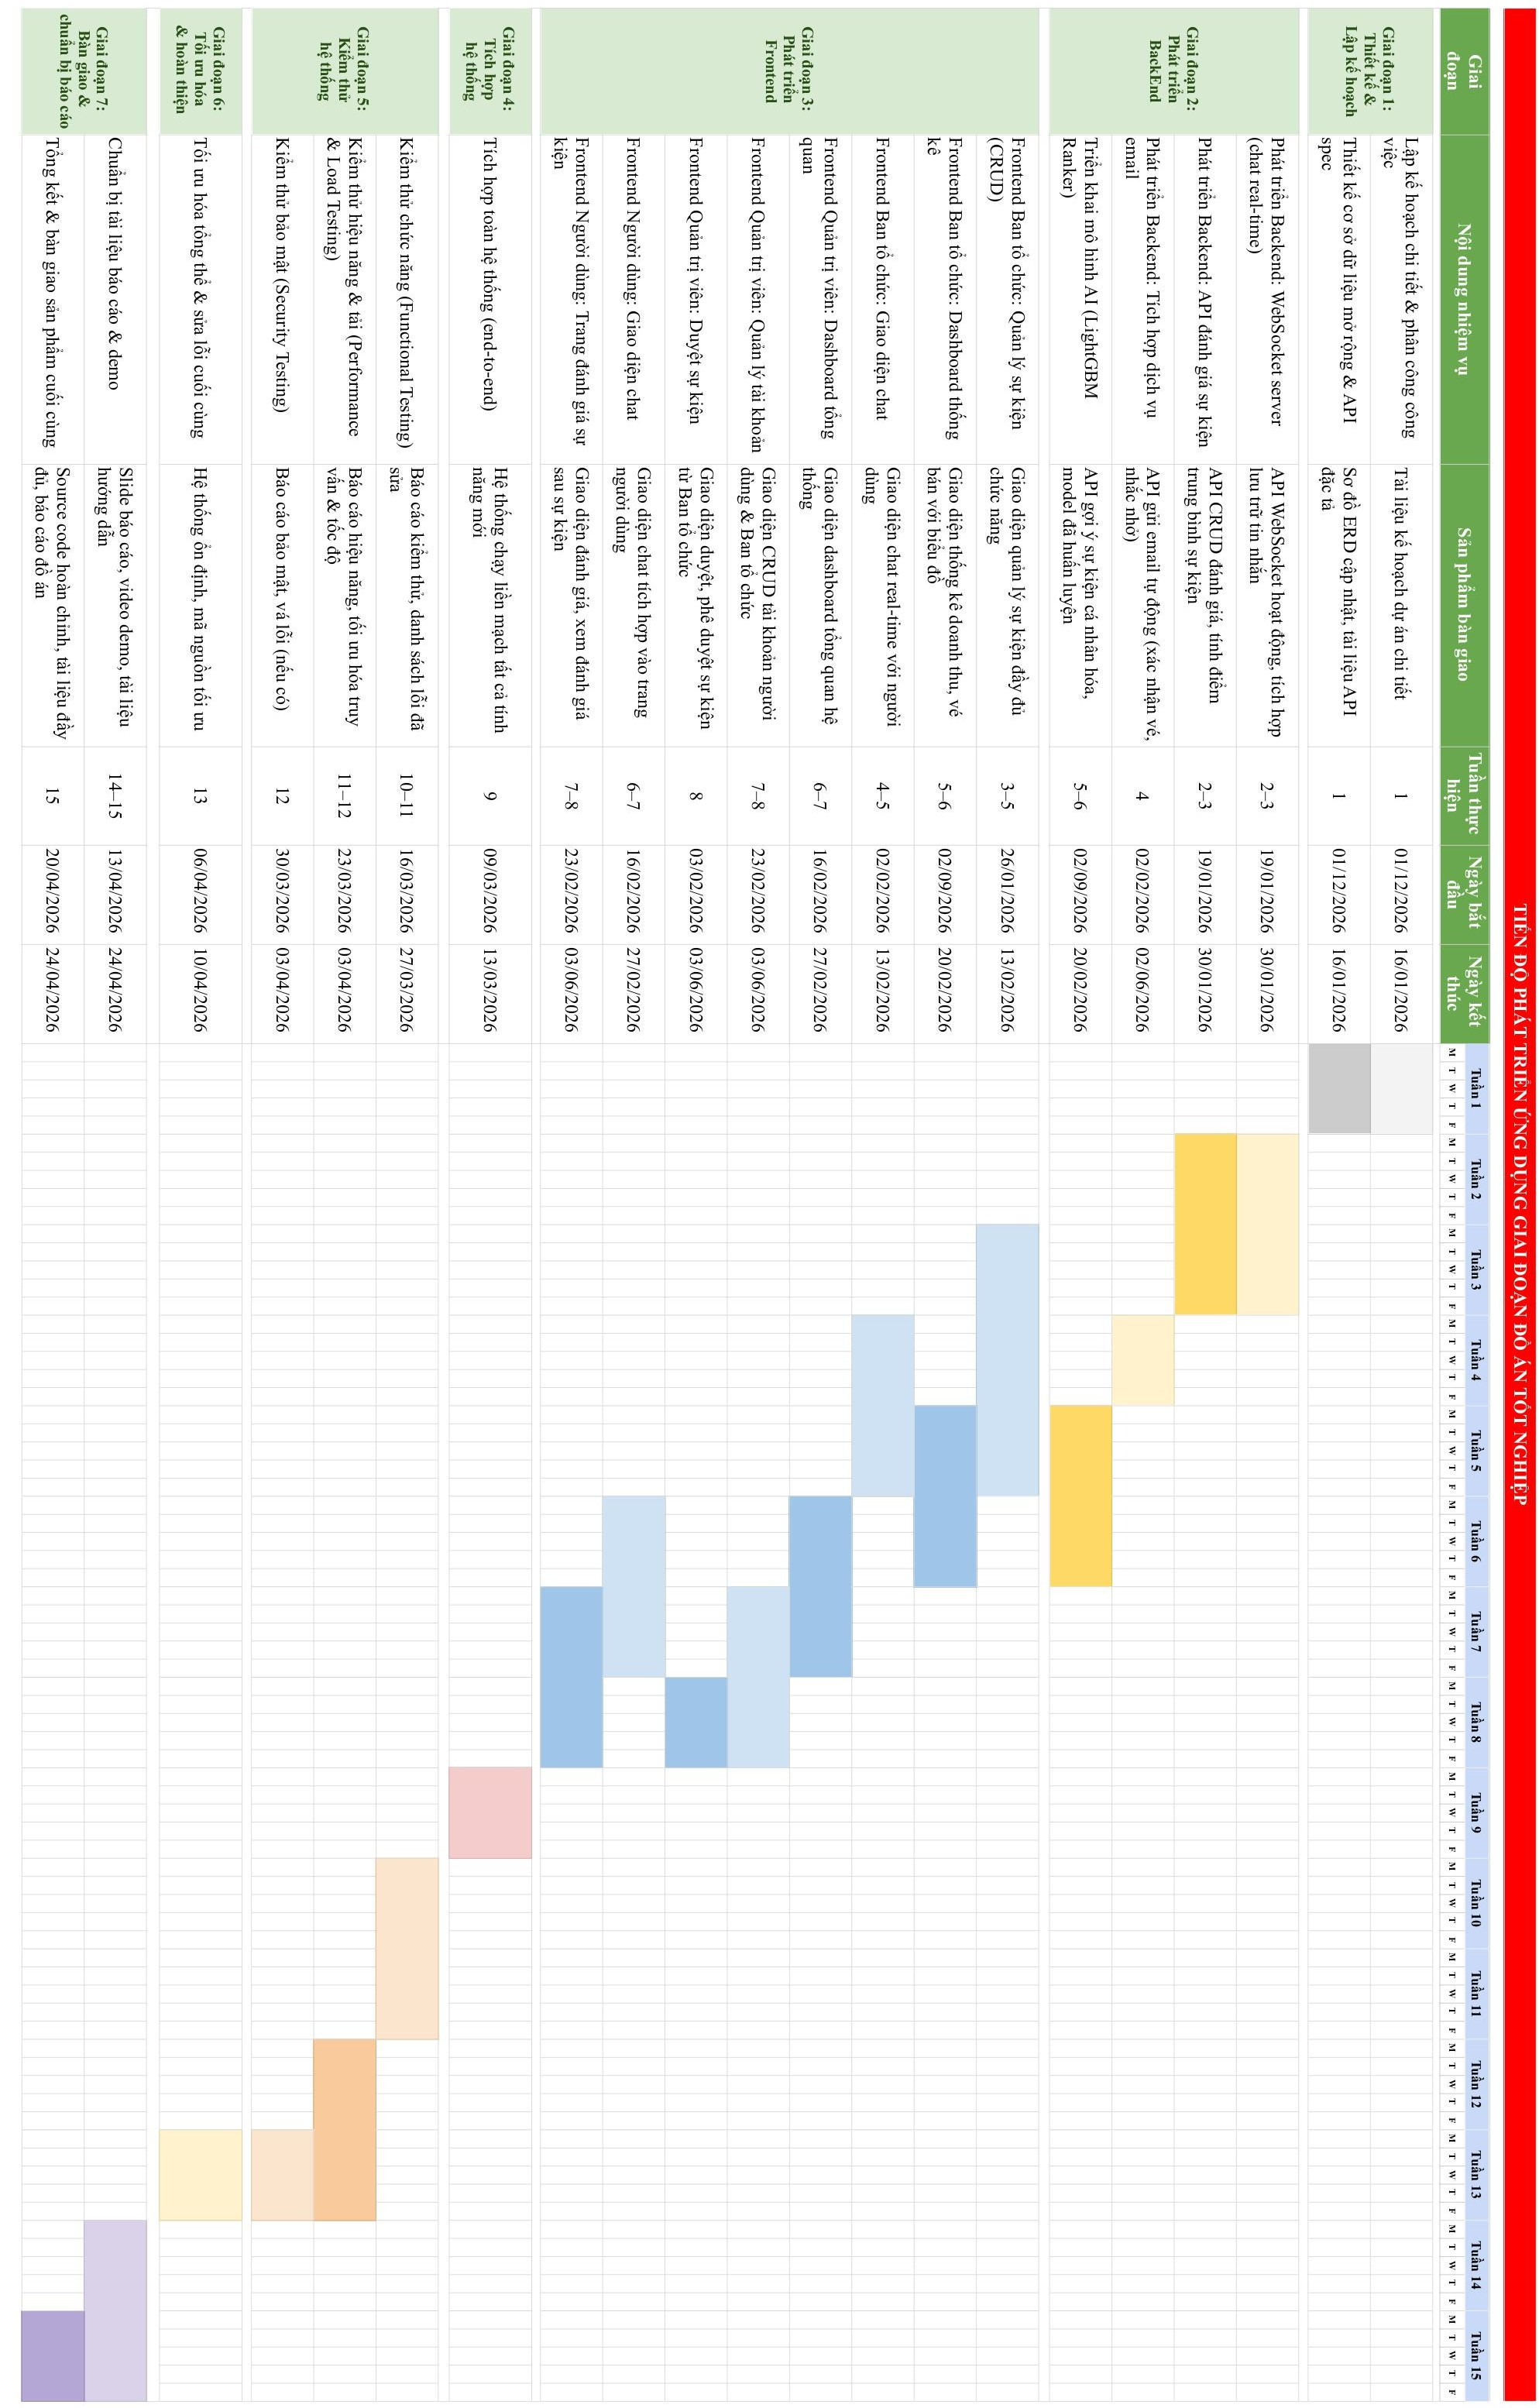
\includegraphics[width=0.95\textwidth]{Images/gantt4.jpg}
    \vspace{15pt}
    \caption{Danh sách công việc và sơ đồ Gantt}
\end{figure}